\documentclass{standalone}
\usepackage{tikz}
\usetikzlibrary{patterns, positioning}
\usetikzlibrary{shapes.misc}
\usepackage[outline]{contour}
\contourlength{1.5pt} 


\begin{document}
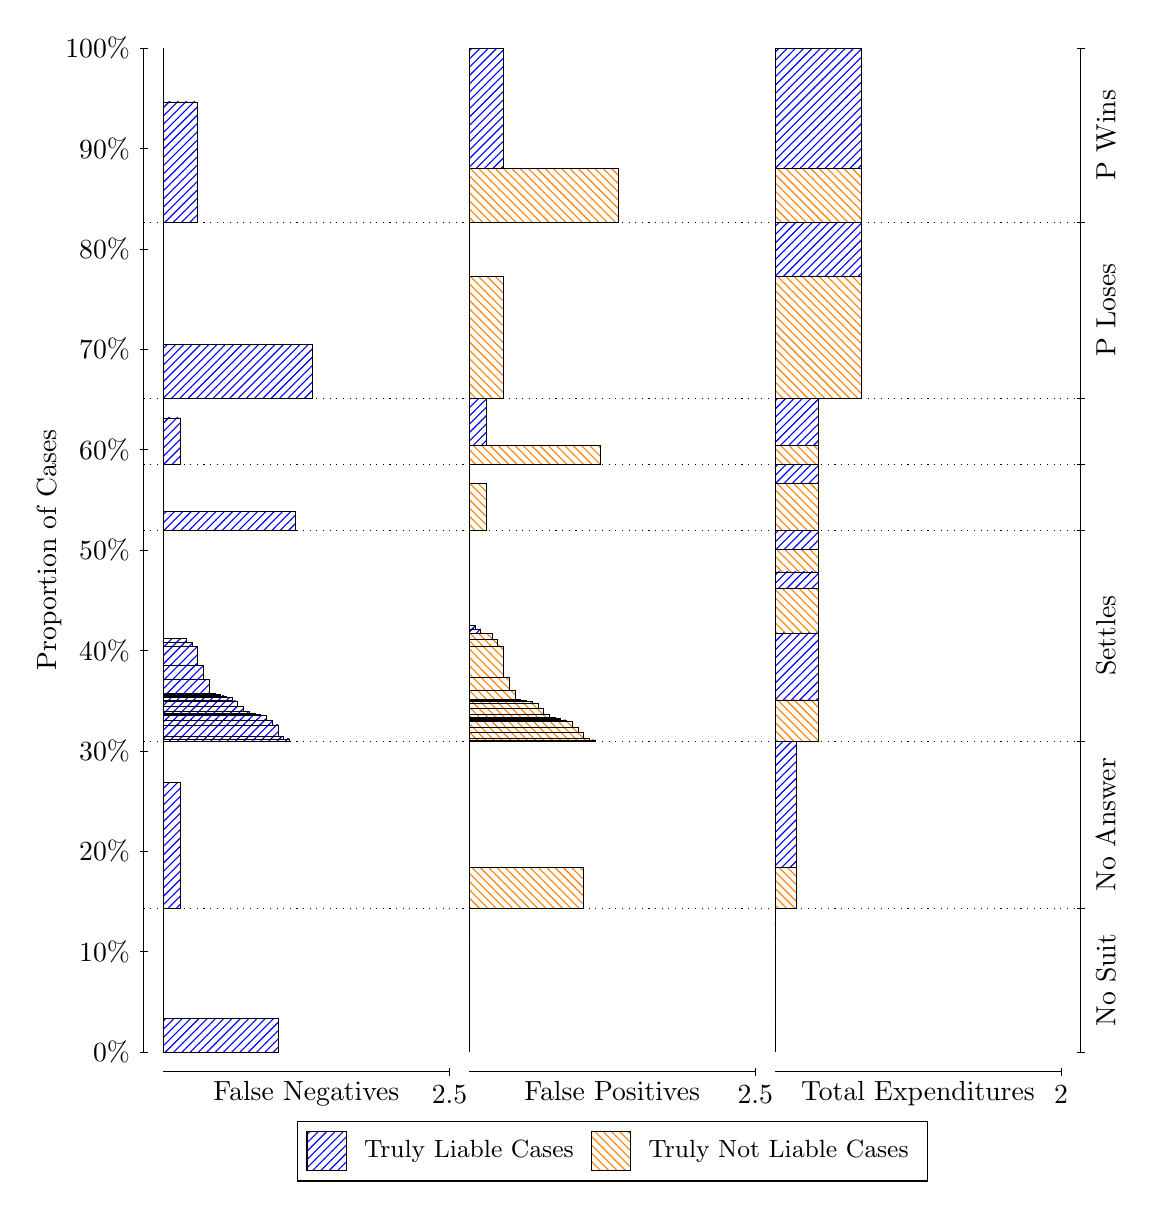
\begin{tikzpicture}
\draw[black, very thin] (1.5,1.75) -- (1.5,14.5);
\node[rotate=90, text=black, anchor=center] at (0.3, 8.125) {Proportion of Cases};
\draw[black, very thin] (1.45,1.75) -- (1.55,1.75);
\node[text=black, anchor=east] at (1.45, 1.75) {0\%};
\draw[black, very thin] (1.45,3.025) -- (1.55,3.025);
\node[text=black, anchor=east] at (1.45, 3.025) {10\%};
\draw[black, very thin] (1.45,4.3) -- (1.55,4.3);
\node[text=black, anchor=east] at (1.45, 4.3) {20\%};
\draw[black, very thin] (1.45,5.575) -- (1.55,5.575);
\node[text=black, anchor=east] at (1.45, 5.575) {30\%};
\draw[black, very thin] (1.45,6.85) -- (1.55,6.85);
\node[text=black, anchor=east] at (1.45, 6.85) {40\%};
\draw[black, very thin] (1.45,8.125) -- (1.55,8.125);
\node[text=black, anchor=east] at (1.45, 8.125) {50\%};
\draw[black, very thin] (1.45,9.4) -- (1.55,9.4);
\node[text=black, anchor=east] at (1.45, 9.4) {60\%};
\draw[black, very thin] (1.45,10.675) -- (1.55,10.675);
\node[text=black, anchor=east] at (1.45, 10.675) {70\%};
\draw[black, very thin] (1.45,11.95) -- (1.55,11.95);
\node[text=black, anchor=east] at (1.45, 11.95) {80\%};
\draw[black, very thin] (1.45,13.225) -- (1.55,13.225);
\node[text=black, anchor=east] at (1.45, 13.225) {90\%};
\draw[black, very thin] (1.45,14.5) -- (1.55,14.5);
\node[text=black, anchor=east] at (1.45, 14.5) {100\%};

\draw[black, very thin] (13.4,1.75) -- (13.4,14.5);
\draw[black, very thin] (13.35,1.75) -- (13.45,1.75);
\node[anchor=west] at (13.35, 1.75) {};
\draw[black, very thin] (13.35,3.5737) -- (13.45,3.5737);
\node[anchor=west] at (13.35, 3.5737) {};
\draw[black, very thin] (13.35,5.6975) -- (13.45,5.6975);
\node[anchor=west] at (13.35, 5.6975) {};
\draw[black, very thin] (13.35,8.3727) -- (13.45,8.3727);
\node[anchor=west] at (13.35, 8.3727) {};
\draw[black, very thin] (13.35,9.208) -- (13.45,9.208);
\node[anchor=west] at (13.35, 9.208) {};
\draw[black, very thin] (13.35,10.053) -- (13.45,10.053);
\node[anchor=west] at (13.35, 10.053) {};
\draw[black, very thin] (13.35,12.289) -- (13.45,12.289);
\node[anchor=west] at (13.35, 12.289) {};
\draw[black, very thin] (13.35,14.5) -- (13.45,14.5);
\node[anchor=west] at (13.35, 14.5) {};

\draw[black, very thin, pattern color=blue, pattern=north east lines] (1.75,1.75) rectangle (3.2033,2.1721);
\draw[black, very thin, pattern color=orange, pattern=north west lines] (1.75,2.1721) rectangle (1.75,3.5737);
\draw[black, very thin, pattern color=blue, pattern=north east lines] (1.75,3.5737) rectangle (1.968,5.174);
\draw[black, very thin, pattern color=orange, pattern=north west lines] (1.75,5.174) rectangle (1.75,5.6975);
\draw[black, very thin, pattern color=blue, pattern=north east lines] (1.75,5.6975) rectangle (3.3487,5.7248);
\draw[black, very thin, pattern color=blue, pattern=north east lines] (1.75,5.7248) rectangle (3.276,5.7588);
\draw[black, very thin, pattern color=blue, pattern=north east lines] (1.75,5.7588) rectangle (3.2033,5.9048);
\draw[black, very thin, pattern color=blue, pattern=north east lines] (1.75,5.9048) rectangle (3.1307,5.9689);
\draw[black, very thin, pattern color=blue, pattern=north east lines] (1.75,5.9689) rectangle (3.058,6.0202);
\draw[black, very thin, pattern color=blue, pattern=north east lines] (1.75,6.0202) rectangle (2.9853,6.0362);
\draw[black, very thin, pattern color=blue, pattern=north east lines] (1.75,6.0362) rectangle (2.9127,6.0435);
\draw[black, very thin, pattern color=blue, pattern=north east lines] (1.75,6.0435) rectangle (2.9127,6.0533);
\draw[black, very thin, pattern color=blue, pattern=north east lines] (1.75,6.0533) rectangle (2.84,6.0799);
\draw[black, very thin, pattern color=blue, pattern=north east lines] (1.75,6.0799) rectangle (2.7673,6.1385);
\draw[black, very thin, pattern color=blue, pattern=north east lines] (1.75,6.1385) rectangle (2.6947,6.2089);
\draw[black, very thin, pattern color=blue, pattern=north east lines] (1.75,6.2089) rectangle (2.622,6.2168);
\draw[black, very thin, pattern color=blue, pattern=north east lines] (1.75,6.2168) rectangle (2.622,6.2535);
\draw[black, very thin, pattern color=blue, pattern=north east lines] (1.75,6.2535) rectangle (2.5493,6.2716);
\draw[black, very thin, pattern color=blue, pattern=north east lines] (1.75,6.2716) rectangle (2.5493,6.2728);
\draw[black, very thin, pattern color=blue, pattern=north east lines] (1.75,6.2728) rectangle (2.4767,6.274);
\draw[black, very thin, pattern color=blue, pattern=north east lines] (1.75,6.274) rectangle (2.4767,6.2868);
\draw[black, very thin, pattern color=blue, pattern=north east lines] (1.75,6.2868) rectangle (2.404,6.2998);
\draw[black, very thin, pattern color=blue, pattern=north east lines] (1.75,6.2998) rectangle (2.3313,6.4864);
\draw[black, very thin, pattern color=blue, pattern=north east lines] (1.75,6.4864) rectangle (2.2587,6.6654);
\draw[black, very thin, pattern color=blue, pattern=north east lines] (1.75,6.6654) rectangle (2.186,6.9028);
\draw[black, very thin, pattern color=blue, pattern=north east lines] (1.75,6.9028) rectangle (2.1133,6.9469);
\draw[black, very thin, pattern color=blue, pattern=north east lines] (1.75,6.9469) rectangle (2.0407,7.0016);
\draw[black, very thin, pattern color=orange, pattern=north west lines] (1.75,7.0016) rectangle (1.75,8.3727);
\draw[black, very thin, pattern color=blue, pattern=north east lines] (1.75,8.3727) rectangle (3.4213,8.6112);
\draw[black, very thin, pattern color=orange, pattern=north west lines] (1.75,8.6112) rectangle (1.75,9.208);
\draw[black, very thin, pattern color=blue, pattern=north east lines] (1.75,9.208) rectangle (1.968,9.8032);
\draw[black, very thin, pattern color=orange, pattern=north west lines] (1.75,9.8032) rectangle (1.75,10.053);
\draw[black, very thin, pattern color=blue, pattern=north east lines] (1.75,10.053) rectangle (3.6393,10.739);
\draw[black, very thin, pattern color=orange, pattern=north west lines] (1.75,10.739) rectangle (1.75,12.289);
\draw[black, very thin, pattern color=blue, pattern=north east lines] (1.75,12.289) rectangle (2.186,13.817);
\draw[black, very thin, pattern color=orange, pattern=north west lines] (1.75,13.817) rectangle (1.75,14.5);
\draw[black, very thin, pattern color=orange, pattern=north west lines] (5.6333,1.75) rectangle (5.6333,3.1516);
\draw[black, very thin, pattern color=blue, pattern=north east lines] (5.6333,3.1516) rectangle (5.6333,3.5737);
\draw[black, very thin, pattern color=orange, pattern=north west lines] (5.6333,3.5737) rectangle (7.0867,4.0972);
\draw[black, very thin, pattern color=blue, pattern=north east lines] (5.6333,4.0972) rectangle (5.6333,5.6975);
\draw[black, very thin, pattern color=orange, pattern=north west lines] (5.6333,5.6975) rectangle (7.232,5.7139);
\draw[black, very thin, pattern color=orange, pattern=north west lines] (5.6333,5.7139) rectangle (7.1593,5.7295);
\draw[black, very thin, pattern color=orange, pattern=north west lines] (5.6333,5.7295) rectangle (7.0867,5.8116);
\draw[black, very thin, pattern color=orange, pattern=north west lines] (5.6333,5.8116) rectangle (7.014,5.8759);
\draw[black, very thin, pattern color=orange, pattern=north west lines] (5.6333,5.8759) rectangle (6.9413,5.9543);
\draw[black, very thin, pattern color=orange, pattern=north west lines] (5.6333,5.9543) rectangle (6.8687,5.9679);
\draw[black, very thin, pattern color=orange, pattern=north west lines] (5.6333,5.9679) rectangle (6.796,5.9814);
\draw[black, very thin, pattern color=orange, pattern=north west lines] (5.6333,5.9814) rectangle (6.796,5.9826);
\draw[black, very thin, pattern color=orange, pattern=north west lines] (5.6333,5.9826) rectangle (6.7233,5.9838);
\draw[black, very thin, pattern color=orange, pattern=north west lines] (5.6333,5.9838) rectangle (6.7233,6.0017);
\draw[black, very thin, pattern color=orange, pattern=north west lines] (5.6333,6.0017) rectangle (6.6507,6.0342);
\draw[black, very thin, pattern color=orange, pattern=north west lines] (5.6333,6.0342) rectangle (6.6507,6.0422);
\draw[black, very thin, pattern color=orange, pattern=north west lines] (5.6333,6.0422) rectangle (6.578,6.1107);
\draw[black, very thin, pattern color=orange, pattern=north west lines] (5.6333,6.1107) rectangle (6.5053,6.1735);
\draw[black, very thin, pattern color=orange, pattern=north west lines] (5.6333,6.1735) rectangle (6.4327,6.1996);
\draw[black, very thin, pattern color=orange, pattern=north west lines] (5.6333,6.1996) rectangle (6.36,6.2156);
\draw[black, very thin, pattern color=orange, pattern=north west lines] (5.6333,6.2156) rectangle (6.2873,6.2176);
\draw[black, very thin, pattern color=orange, pattern=north west lines] (5.6333,6.2176) rectangle (6.2873,6.2303);
\draw[black, very thin, pattern color=orange, pattern=north west lines] (5.6333,6.2303) rectangle (6.2147,6.3375);
\draw[black, very thin, pattern color=orange, pattern=north west lines] (5.6333,6.3375) rectangle (6.142,6.5054);
\draw[black, very thin, pattern color=orange, pattern=north west lines] (5.6333,6.5054) rectangle (6.0693,6.9083);
\draw[black, very thin, pattern color=orange, pattern=north west lines] (5.6333,6.9083) rectangle (5.9967,6.9907);
\draw[black, very thin, pattern color=orange, pattern=north west lines] (5.6333,6.9907) rectangle (5.924,7.0686);
\draw[black, very thin, pattern color=blue, pattern=north east lines] (5.6333,7.0686) rectangle (5.7787,7.1233);
\draw[black, very thin, pattern color=blue, pattern=north east lines] (5.6333,7.1233) rectangle (5.706,7.1674);
\draw[black, very thin, pattern color=blue, pattern=north east lines] (5.6333,7.1674) rectangle (5.6333,8.3727);
\draw[black, very thin, pattern color=orange, pattern=north west lines] (5.6333,8.3727) rectangle (5.8513,8.9694);
\draw[black, very thin, pattern color=blue, pattern=north east lines] (5.6333,8.9694) rectangle (5.6333,9.208);
\draw[black, very thin, pattern color=orange, pattern=north west lines] (5.6333,9.208) rectangle (7.3047,9.4574);
\draw[black, very thin, pattern color=blue, pattern=north east lines] (5.6333,9.4574) rectangle (5.8513,10.053);
\draw[black, very thin, pattern color=orange, pattern=north west lines] (5.6333,10.053) rectangle (6.0693,11.603);
\draw[black, very thin, pattern color=blue, pattern=north east lines] (5.6333,11.603) rectangle (5.6333,12.289);
\draw[black, very thin, pattern color=orange, pattern=north west lines] (5.6333,12.289) rectangle (7.5227,12.972);
\draw[black, very thin, pattern color=blue, pattern=north east lines] (5.6333,12.972) rectangle (6.0693,14.5);
\draw[black, very thin, pattern color=orange, pattern=north west lines] (9.5167,1.75) rectangle (9.5167,3.1516);
\draw[black, very thin, pattern color=blue, pattern=north east lines] (9.5167,3.1516) rectangle (9.5167,3.5737);
\draw[black, very thin, pattern color=orange, pattern=north west lines] (9.5167,3.5737) rectangle (9.7892,4.0972);
\draw[black, very thin, pattern color=blue, pattern=north east lines] (9.5167,4.0972) rectangle (9.7892,5.6975);
\draw[black, very thin, pattern color=orange, pattern=north west lines] (9.5167,5.6975) rectangle (10.062,6.2205);
\draw[black, very thin, pattern color=blue, pattern=north east lines] (9.5167,6.2205) rectangle (10.062,7.0723);
\draw[black, very thin, pattern color=orange, pattern=north west lines] (9.5167,7.0723) rectangle (10.062,7.6376);
\draw[black, very thin, pattern color=blue, pattern=north east lines] (9.5167,7.6376) rectangle (10.062,7.847);
\draw[black, very thin, pattern color=orange, pattern=north west lines] (9.5167,7.847) rectangle (10.062,8.13);
\draw[black, very thin, pattern color=blue, pattern=north east lines] (9.5167,8.13) rectangle (10.062,8.3727);
\draw[black, very thin, pattern color=orange, pattern=north west lines] (9.5167,8.3727) rectangle (10.062,8.9694);
\draw[black, very thin, pattern color=blue, pattern=north east lines] (9.5167,8.9694) rectangle (10.062,9.208);
\draw[black, very thin, pattern color=orange, pattern=north west lines] (9.5167,9.208) rectangle (10.062,9.4574);
\draw[black, very thin, pattern color=blue, pattern=north east lines] (9.5167,9.4574) rectangle (10.062,10.053);
\draw[black, very thin, pattern color=orange, pattern=north west lines] (9.5167,10.053) rectangle (10.607,11.603);
\draw[black, very thin, pattern color=blue, pattern=north east lines] (9.5167,11.603) rectangle (10.607,12.289);
\draw[black, very thin, pattern color=orange, pattern=north west lines] (9.5167,12.289) rectangle (10.607,12.972);
\draw[black, very thin, pattern color=blue, pattern=north east lines] (9.5167,12.972) rectangle (10.607,14.5);
\draw[black, dotted] (1.5,3.5737) -- (13.4,3.5737);
\draw[black, dotted] (1.5,5.6975) -- (13.4,5.6975);
\draw[black, dotted] (1.5,8.3727) -- (13.4,8.3727);
\draw[black, dotted] (1.5,9.208) -- (13.4,9.208);
\draw[black, dotted] (1.5,10.053) -- (13.4,10.053);
\draw[black, dotted] (1.5,12.289) -- (13.4,12.289);
\draw[black, very thin] (1.75,1.5) -- (5.3833,1.5);
\node[text=black, anchor=north] at (3.5667, 1.5) {False Negatives};
\draw[black, very thin] (5.3833,1.45) -- (5.3833,1.55);
\node[text=black, anchor=north] at (5.3833, 1.45) {2.5};

\draw[black, very thin] (5.6333,1.5) -- (9.2667,1.5);
\node[text=black, anchor=north] at (7.45, 1.5) {False Positives};
\draw[black, very thin] (9.2667,1.45) -- (9.2667,1.55);
\node[text=black, anchor=north] at (9.2667, 1.45) {2.5};

\draw[black, very thin] (9.5167,1.5) -- (13.15,1.5);
\node[text=black, anchor=north] at (11.333, 1.5) {Total Expenditures};
\draw[black, very thin] (13.15,1.45) -- (13.15,1.55);
\node[text=black, anchor=north] at (13.15, 1.45) {2};

\node[text=black, centered, rotate=90] at (13.72, 2.6619) {\contour{white}{No Suit}};
\node[text=black, centered, rotate=90] at (13.72, 4.6356) {\contour{white}{No Answer}};
\node[text=black, centered, rotate=90] at (13.72, 7.0351) {\contour{white}{Settles}};


\node[text=black, centered, rotate=90] at (13.72, 11.171) {\contour{white}{P Loses}};
\node[text=black, centered, rotate=90] at (13.72, 13.395) {\contour{white}{P Wins}};

\draw (7.449999999999999,1.5) node[draw=none] (baseCoordinate) {};
\begin{scope}[align=center]
        \matrix[scale=0.5, draw=black, below=0.5cm of baseCoordinate, nodes={draw}, column sep=0.1cm]{
            \node[rectangle, draw, minimum width=0.5cm, minimum height=0.5cm, pattern color=blue, pattern=north east lines] {}; &
            \node[draw=none, font=\small, text=black] (B) {Truly Liable Cases}; &
            \node[rectangle, draw, minimum width=0.5cm, minimum height=0.5cm, pattern color=orange, pattern=north west lines] {}; &
            \node[draw=none, font=\small, text=black] (B) {Truly Not Liable Cases}; \\
            };
\end{scope}

\end{tikzpicture}
\end{document}